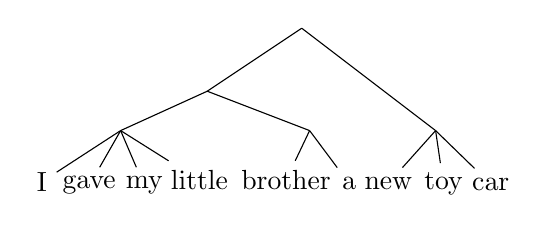
\begin{tikzpicture}
\node (I) at (1,0.05) {I};
\node (gave) at (1.6,0) {gave};
\node (my) at (2.3,0) {my};
\node (little) at (3.0,0.07) {little};
\node (brother) at (4.1,.07) {brother};
\node (a) at (4.9,0.03) {a};
\node (new) at (5.4,0.03) {new};
\node (toy) at (6.1,0.02) {toy};
\node (car) at (6.7,0.02) {car};

\coordinate (Igavemylittle) at (2,0.7);
\coordinate (brothera) at (4.4,0.7);
\coordinate(newtoycar) at (6.0,0.7);
\coordinate (all) at (4.3,2);
\coordinate (Igavemybrothera) at (3.1, 1.2);

\foreach \from/\to in {Igavemylittle/I, Igavemylittle/gave, Igavemylittle/my, Igavemylittle/little, a/brothera, brother/brothera, newtoycar/new, newtoycar/toy, newtoycar/car, Igavemybrothera/Igavemylittle, Igavemybrothera/brothera, all/newtoycar, all/Igavemybrothera}
	\draw (\from) -- (\to);

\end{tikzpicture}
\caption{A tree that describe how the sentence 'I gave my little brother a new toy car' could have been compositionally constructed.}\label{fig:struct1}